\section{Matched-history design and evaluation objects}

\subsection{Primary task family: MHST}

We study revisability with \textbf{Matched-History Suspect Tracking} (MHST), a synthetic controlled task designed to separate current designated state from the path that produced it. Each world contains four suspect profiles, each defined by five unique attributes. Prefix clues map unambiguously to one suspect profile. From each base world we generate a \emph{fresh} prefix and a \emph{committed} prefix with the same designated incumbent/challenger pair and the same designated evidence margin $m\in\{1,2,3\}$, but with different evidence order. The history-depth parameter $k\in\{0,1,2\}$ controls how much challenger-consistent prefix evidence is present. After the prefix, a fixed six-slot late packet adds challenger evidence at dose $d\in\{0,\ldots,6\}$.

The primary evaluation uses Qwen2.5-7B-Instruct on held-out MHST test pairs. Auxiliary checks use Llama-3.1-8B on MHST and Qwen2.5-7B on RC-ICL. Those auxiliary settings are reported honestly but are not treated as co-equal main results.

\begin{figure}[t]
    \centering
    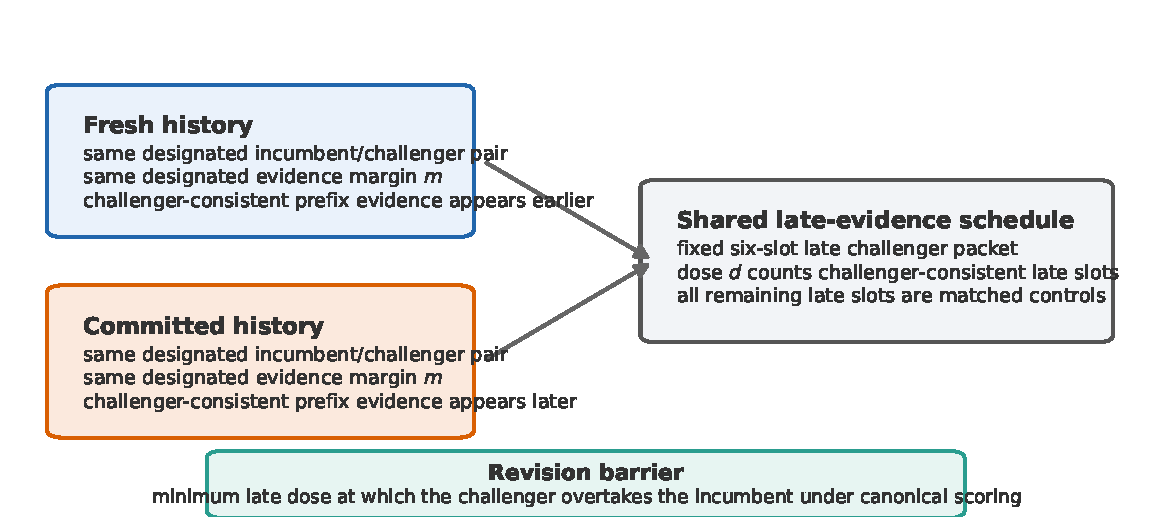
\includegraphics[width=\linewidth]{figures/figure1_matched_history_schematic.pdf}
    \caption{Matched-history construction. Fresh and committed prefixes are matched on the designated incumbent/challenger pair and designated evidence margin, then exposed to the same late challenger-evidence schedule. The behavioral question is whether the same designated state is equally revisable once later counterevidence arrives.}
    \label{fig:matched-history}
\end{figure}

Figure~\ref{fig:matched-history} shows the logic: the paper is about \emph{matching designated state while varying history}. That distinction is critical. The stronger phrase ``same current leader'' is reserved for the leader-consistent subset $\Slead$, defined by prefix-only canonical scoring, and is never used globally.

\subsection{Barrier, reversibility, and paired summaries}

For a prefix $p$, let $q_h(p\oplus U_d)$ denote the canonical score assigned to hypothesis $h$ after appending the late packet $U_d$ at dose $d$. The raw revision barrier is
\begin{equation}
    \Braw(p) = \min\{d\in\{0,\ldots,6\}: q_{\text{challenger}}(p\oplus U_d) \ge q_{\text{incumbent}}(p\oplus U_d)\},
\end{equation}
with $\Braw(p)=\infty$ if no dose flips the ordering. The main scalar summary clips this to
\begin{equation}
    \Bcap(p) = \min(\Braw(p), 7),
\end{equation}
and the paired history effect is
\begin{equation}
    \DeltaBpair(p) = \Bcap(p_{\text{committed}}) - \Bcap(p_{\text{fresh}}).
\end{equation}
Positive values mean that the committed member of a matched pair requires more late challenger evidence to reverse.

We also retain the full reversibility curve
\begin{equation}
    R(d) = \Pr[\Braw \le d],
\end{equation}
and one bounded companion summary based on raw barriers:
\begin{equation}
    \MeanFlip(e) = \frac{1}{7}\sum_{d=0}^{6} \mathbb{1}[\Braw(e) \le d],
\end{equation}
with paired gap $\DeltaMeanFlip = \MeanFlip(\text{fresh}) - \MeanFlip(\text{committed})$.

\subsection{Validity filters and control ladder}

Main behavioral summaries use the paired-valid subset $\validpair$, where neither member of a pair is invalidated by distractor takeover. Stronger same-current-leader wording is reserved for the leader-consistent subset $\Slead$, defined by prefix-only canonical scoring rather than by generation. The behavioral story is further constrained by a required $k{=}0$ null cell, a locked output-margin control, and a no-conflict sanity check that exceeds the project's threshold on MHST/Qwen.

\begin{tcolorbox}[colback=softgreen,colframe=residual!60!black,boxrule=0.8pt,arc=2pt,left=8pt,right=8pt,top=6pt,bottom=6pt]
\textbf{State-only insufficiency proposition.} Consider any account that predicts revisability solely from current-state summaries such as designated margin and prefix-only output margin. In the operational setting of this paper, once designated incumbent/challenger state is matched and those summaries are accounted for, the expected fresh-versus-committed paired gap should vanish. The state-only decomposition in Section~\ref{sec:state-only} tests exactly that implication: the state-only predicted paired gap is the part attributed to current-state summaries alone, and the residual paired gap is the remaining history effect. A positive residual therefore rejects that class of state-only accounts for this matched-history setting.
\end{tcolorbox}
